Para el desarrollo de un sistema de visión estereoscópica, es necesario realizar un correcto procesamiento de imágenes digitales, acompañado de un sistema confiable y robusto que pueda evaluar los posibles escenarios, y trasladar sus decisiones al mundo real mediante actuadores correctamente controlados.

\subsection{Control Difuso}

El control difuso está basado en lógica borrosa, que permite tratar información imprecisa en término de conjuntos difusos, estos conjuntos de combinan en reglas para definir acciones, y permiten manipular valores lingüísticos poco definidos como (mucho, poco, alto, bajo, cerca, caliente, etc). La teoría de conjuntos borrosos parte de la teoría clásica de conjuntos, añadiendo un grado de pertenencia definido como un número real entre 0 y 1. En la figura \ref{fig:conjunto_difuso} puede verse un ejemplo de la definición de conjuntos difusos para la variable estatura.

\begin{figure}[b]
	\begin{center}
		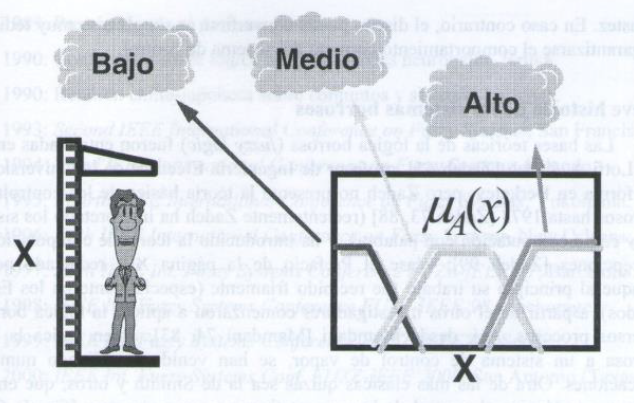
\includegraphics[width=0.49\textwidth]{images/ejemplocd.png}\\
		\caption{Ejemplo de conjuntos difusos para la variable estatura.}\label{fig:conjunto_difuso}
	\end{center}
\end{figure}

La base de reglas difusas en control está dada por una colección de reglas $R$ con el formato de la que puede verse en \ref{eq:regla_difuso} Este formato es conocido como borroso puro o tipo Mamdani.

\begin{equation} \label{eq:regla_difuso}
	R: \;\: IF\; x_{1}\; is\; F_{1}\; and...\, and\, x_{n}\; is\; F_{n}\; THEN\; y=f
\end{equation}

Todo controlador difuso está definido por tres pasos fundamentales\
\begin{enumerate}
	\item \textbf{Borrosificar:} Consiste en convertir lo valores no difusos de las variables a controlar, y obtener los grados de pertenencia a cada uno de los conjuntos difusos definidos.
	
	\item \textbf{Inferir:} Consiste en realizar la inferencia a partir de las reglas que definen el sistema de control.
	
	\item \textbf{Desborrosificar:} Consiste es convertir lo valores obtenidos en la inferencias para aplicarlo como control de algún actuador.
\end{enumerate}

\begin{figure}[h]
	\begin{center}
		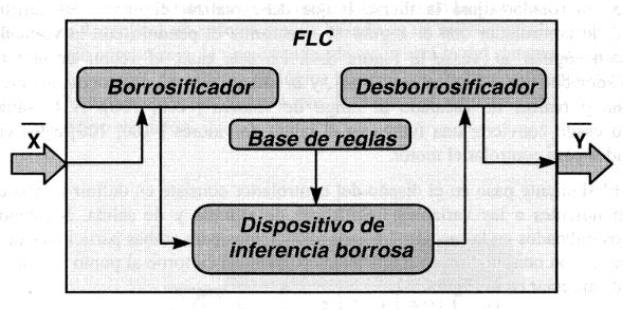
\includegraphics[width=0.47\textwidth]{images/controlado.png}\\
		\caption{Estructura de un controlador difuso.}\label{fig:controlador_difuso}
	\end{center}
\end{figure}

\subsection{Procesador de señales digitales (DSP)}

Al implementar visión artificial en vehículos autónomos, se debe tener en cuenta que estos funcionan mediante procesamiento de imágenes proyectadas por el mismo entorno que lo rodea, es una técnica de procesamiento automático para comprender la complejidad y los pasos a realizar. Hay más tecnologías, pero todas buscan las mismas cosas y determinan patrones. Como por ejemplo hace solo unos años, la gente decidió marcar manualmente las imágenes para mostrar a la máquina dónde estaban las orejas o la cola de un gato. Esto se llama ``función manual'' y alguna vez se usó ampliamente, pero requiere mucho tiempo y es puramente ``comparativo''. Para este ejercicio se plantea utilizar algoritmos para generar un mapa de disparidad binocular para inferir la tridimensionalidad de una escena. En la figura \ref{fig:dsp_stereo} puede verse un ejemplo del resultado que se pretende obtener en este proceso.

\begin{figure}[h]
	\begin{center}
		\begin{subfigure}{0.49\textwidth}
			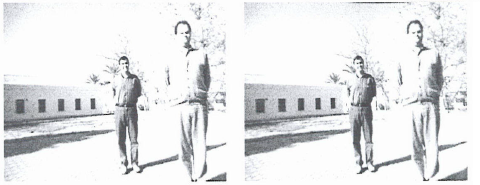
\includegraphics[width=\textwidth]{images/imgestereo.png}
			\caption{Par de imágenes estéreo.}
		\end{subfigure}
		\begin{subfigure}{0.49\textwidth}
			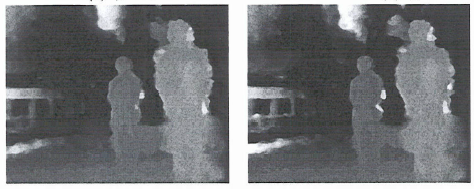
\includegraphics[width=\textwidth]{images/res.png}
			\caption{Resultados obtenidos.}
		\end{subfigure}
	\end{center}
	\caption{Ejemplo de mapa de disparidad}\label{fig:dsp_stereo}
\end{figure}

\subsection{Inteligencia Artificial}

Se considera búsquedas heurísticas, a los algoritmos que utilizan conocimiento específico del problema más allá de la definición del problema en sí mismo, esta basada generalidades de BÚSQUEDA-ÁRBOLES o de BÚSQUEDA-GRAFOS en el cual se selecciona un nodo para la expansión basada en una función de evaluación, denominada heurística $h(n)$ que hace referencia al coste estimado del camino más barato desde el nodo n a un nodo objetivo. Gracias a esto puede encontrarse soluciones de una manera más eficiente.

\paragraph{Ejemplo de Código en Java}
Aquí hay un ejemplo de cómo se podría incluir código Java utilizando el paquete \texttt{listings}:

\begin{lstlisting}[language=Java, caption=Ejemplo de cálculo de heurística A*, label=lst:a-star-heuristic]
// Función heurística para el algoritmo A*
public double calculateHeuristic(Node current, Node goal) {
    // Distancia Euclidiana como ejemplo
    double dx = current.getX() - goal.getX();
    double dy = current.getY() - goal.getY();
    return Math.sqrt(dx*dx + dy*dy);
}
\end{lstlisting}

A la forma más ampliamente conocida de la búsqueda heurística se le llama algoritmo	A* (A estrella). Evalúa los nodos combinando $g(n)$, el coste para alcanzar el nodo, y $h(n)$, el coste de ir al nodo objetivo:

\begin{equation} \label{eq:heuristica}
	f(n)=g(n)+h(n)
\end{equation}

La base de reglas difusas en control está dada por una colección de reglas $R$ con el formato de la que puede verse en \ref{eq:regla_difuso} Este formato es conocido como borroso puro o tipo Mamdani.

\begin{equation} \label{eq:regla_difuso}
	R: \;\: IF\; x_{1}\; is\; F_{1}\; and...\, and\, x_{n}\; is\; F_{n}\; THEN\; y=f
\end{equation}

Todo controlador difuso está definido por tres pasos fundamentales\
\begin{enumerate}
	\item \textbf{Borrosificar:} Consiste en convertir lo valores no difusos de las variables a controlar, y obtener los grados de pertenencia a cada uno de los conjuntos difusos definidos.
	
	\item \textbf{Inferir:} Consiste en realizar la inferencia a partir de las reglas que definen el sistema de control.
	
	\item \textbf{Desborrosificar:} Consiste es convertir lo valores obtenidos en la inferencias para aplicarlo como control de algún actuador.
\end{enumerate}

\begin{figure}[h]
	\begin{center}
		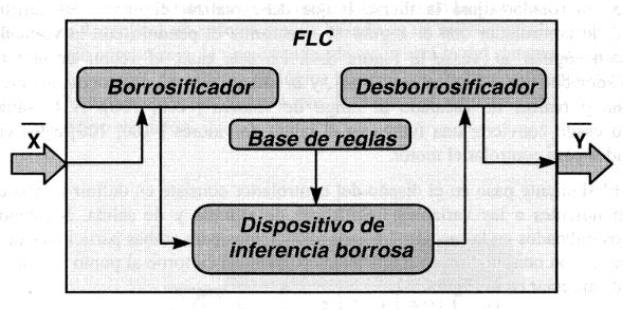
\includegraphics[width=0.47\textwidth]{images/controlado.png}\\
		\caption{Estructura de un controlador difuso \cite{ref:controlador}.}\label{e}
	\end{center}
\end{figure}

La base de reglas difusas en control está dada por una colección de reglas $R$ con el formato de la que puede verse en \ref{eq:regla} Este formato es conocido como borroso puro o tipo Mamdani.

\begin{equation} \label{eq:regla}
	R: \;\: IF\; x_{1}\; is\; F_{1}\; and...\, and\, x_{n}\; is\; F_{n}\; THEN\; y=f
\end{equation}

Todo controlador difuso está definido por tres pasos fundamentales\
\begin{enumerate}
	\item \textbf{Borrosificar:} Consiste en convertir lo valores no difusos de las variables a controlar, y obtener los grados de pertenencia a cada uno de los conjuntos difusos definidos.
	
	\item \textbf{Inferir:} Consiste en realizar la inferencia a partir de las reglas que definen el sistema de control.
	
	\item \textbf{Desborrosificar:} Consiste es convertir lo valores obtenidos en la inferencias para aplicarlo como control de algún actuador.
\end{enumerate}

\begin{figure}[h]
	\begin{center}
		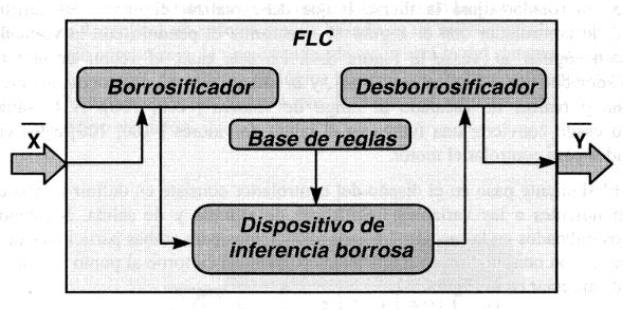
\includegraphics[width=0.47\textwidth]{images/controlado.png}\\
		\caption{Estructura de un controlador difuso \cite{controlador}.}\label{e}
	\end{center}
\end{figure}

\subsection{Procesador de señales digitales (DSP)}

Al implementar visión artificial en vehículos autónomos, se debe tener en cuenta que estos funcionan mediante procesamiento de imágenes proyectadas por el mismo entorno que lo rodea, es una técnica de procesamiento automático para comprender la complejidad y los pasos a realizar. Hay más tecnologías, pero todas buscan las mismas cosas y determinan patrones. Como por ejemplo hace solo unos años, la gente decidió marcar manualmente las imágenes para mostrar a la máquina dónde estaban las orejas o la cola de un gato. Esto se llama ``función manual'' y alguna vez se usó ampliamente, pero requiere mucho tiempo y es puramente ``comparativo''\cite{dsp}. Para este ejercicio se plantea utilizar algoritmos para generar un mapa de disparidad binocular para inferir la tridimensionalidad de una escena. En la figura \ref{ejemdsp} puede verse un ejemplo del resultado que se pretende obtener en este proceso.

\begin{figure}[h]
	\begin{center}
		\begin{subfigure}{0.49\textwidth}
			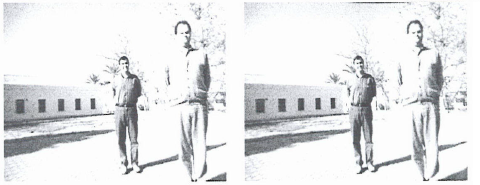
\includegraphics[width=\textwidth]{images/imgestereo.png}
			\caption{Par de imágenes estéreo.}
		\end{subfigure}
		\begin{subfigure}{0.49\textwidth}
			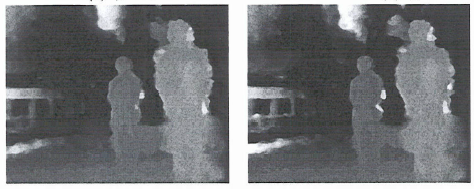
\includegraphics[width=\textwidth]{images/res.png}
			\caption{Resultados obtenidos.}
		\end{subfigure}
	\end{center}
	\caption{Ejemplo de mapa de disparidad \cite{disparidad}}\label{ejemdsp}
\end{figure}

\subsection{Inteligencia Artificial}

Se considera búsquedas heurísticas, a los algoritmos que utilizan conocimiento específico del problema más allá de la definición del problema en sí mismo, esta basada generalidades de BÚSQUEDA-ÁRBOLES o de BÚSQUEDA-GRAFOS en el cual se selecciona un nodo para la expansión basada en una función de evaluación, denominada heurística $h(n)$ que hace referencia al coste estimado del camino más barato desde el nodo n a un nodo objetivo. Gracias a esto puede encontrarse soluciones de una manera más eficiente.

\paragraph{Ejemplo de Código en Java}
Aquí hay un ejemplo de cómo se podría incluir código Java utilizando el paquete \texttt{listings}:

\begin{lstlisting}[language=Java, caption=Ejemplo de cálculo de heurística A*, label=lst:a-star-heuristic]
// Función heurística para el algoritmo A*
public double calculateHeuristic(Node current, Node goal) {
    // Distancia Euclidiana como ejemplo
    double dx = current.getX() - goal.getX();
    double dy = current.getY() - goal.getY();
    return Math.sqrt(dx*dx + dy*dy);
}
\end{lstlisting}
A la forma más ampliamente conocida de la búsqueda heurística se le llama algoritmo	A* (A estrella). Evalúa los nodos combinando $g(n)$, el coste para alcanzar el nodo, y $h(n)$, el coste de ir al nodo objetivo:

\begin{equation} \label{eq:heuristica}
	f(n)=g(n)+h(n)
\end{equation}